\documentclass[12pt]{article}

\usepackage{sbc-template}
\usepackage{float}
\usepackage{graphicx,url}
\usepackage[utf8]{inputenc}
\usepackage[brazil]{babel}
\usepackage[latin1]{inputenc}  
%\usepackage{hyperref}

\sloppy

\title{Modelo de Aprendizado de Máquina para\\ Classificação de Tipos de Pokémons}

\author{Filipe Henrique Pereira Barbosa\inst{1}, Jeremias de Jesus Fernandes Ventura\inst{1},\\Julio Cesar da Silva Rodrigues\inst{1}}


\address{Departamento de Ciência da Computação -- Universidade Federal de São João del-Rei
  (UFSJ)\\
  36.301-360 -- São João del-Rei -- MG -- Brazil
  \email{jeremiassfernandes@hotmail.com, filipevp13@gmail.com,}
  \email{julio.csr.271@aluno.ufsj.edu.br}
}

\begin{document} 

\maketitle

\begin{abstract}
 
 In this article, we describe a project based on the construction of a machine learning model, capable of classifying pokémons. The core idea consists of utilize, with specific programming libraries assistance, machine learning methods, which includes the decision tree, random forest and gradient boosting. All this allied with a few basic pre-processing techniques to perform predictions on the primary type that any pokémon has, given it's features.
 
\end{abstract}
     
\begin{resumo} 
  
Neste artigo, nós descrevemos um trabalho sobre a construção de um modelo de aprendizado de máquina para classificação de pokémons. A ideia principal consiste em utilizar, com o auxílio de bibliotecas de programação, métodos de aprendizado de máquina que incluem árvore de decisão, floresta aleatória e gradient boosting, aliados à algumas técnicas básicas de pré-processamento para predizer o tipo primário de um pokémon, dadas as suas características. 

\end{resumo}

\section{Introdução}

O anime Pokémon fez parte de boa parte da infância dos jovens/adultos de hoje. Dentro do universo deste anime, existem animais chamados pokémons. O anime conta a história de um treinador de pokémons chamado Ash Katchum, e exibe sua jornada em busca de se tornar um Mestre Pokémon.

Neste anime, os pokémons possuem poderes e habilidades que usam em lutas entre seus Mestres Pokémons. Seu conjunto de habilidades e poderes são difinidos de acordo com seu tipo Pokémon. Existem no total 18 tipos diferentes de pokémons. Cada pokémon possui no mínimo dois tipos distintos, sendo um primário e o(s) outro(s) secundário(s).

Este estudo visa a construção de um modelo de Aprendizado de Máquina supervisionado baseado no método de Árvore de Decisão, cujo qual servirá para predizer qual o tipo dominante de determinado pokémon, dadas as suas características. 

\section{Fundamentação Teórica} 

Nas subseções subsequentes, serão explanados de forma breve, métodos e conceitos que foram abordados à todo momento no desenvolvimento deste trabalho.

\subsection{Aprendizado de Máquina}

Aprendizado de Máquina é uma área de pesquisa da Inteligência Artificial que visa o desenvolvimento de softwares que possuam a capacidade de aprender a executar uma dada tarefa com sua própria experiência, ou seja, de forma autônoma, sem qualquer necessidade de intervenções humanas \cite{Cerri:06}.

Esses algoritmos podem realizar previsões com base em amostras, ou tomar decisões com base apenas em dados previamente coletados (dados pra treino), obtendo altas taxas de acerto no caso de uma formulação adequada do modelo de aprendizado.

\subsection{Árvore de Decisão}

As Árvores de Decisão são um dos modelos mais simples e usados em inferência indutiva. Este método representa funções como árvores de decisão. Estas árvores são treinadas de acordo com um conjunto de treino (exemplos previamente classificados) e posteriormente, outros exemplos são classificados de acordo com essa mesma árvore. Para a construção destas árvores são usados algoritmos como o ID3 \cite{ID3} e C4.5 \cite{C45}.

\subsubsection{Estrutura de uma Árvore de Decisão}

De acordo com Marcelo S. Lauretto \cite{Lauretto:06}, as árvores de decisão (Figura~\ref{fig:exampleFig1}) possuem a seguinte estrutura:

\begin{itemize}
    \item Um nó folha (ou nó resposta) que contém o nome de uma classe ou o símbolo nulo (nulo indica que não é possível atribuir nenhuma classe ao nó por não haver nenhum exemplo que corresponda a esse nó);
    \item Um nó interno (ou nó de decisão) que contém o nome de um atributo; para cada possível valor do atributo, corresponde um ramo para uma outra árvore de decisão.
\end{itemize}

\noindent Logo, uma árvore de decisão comum possui a seguinte estrutura típica:

\begin{itemize}
    \item Nós internos que são rotulados com atributos;
    \item Folhas que são rotuladas com classes;
    \item Ramos que são rotulados com valores (atributos categóricos) ou com intervalos (atributos numéricos).
\end{itemize}

\begin{figure}[ht]
    \centering
    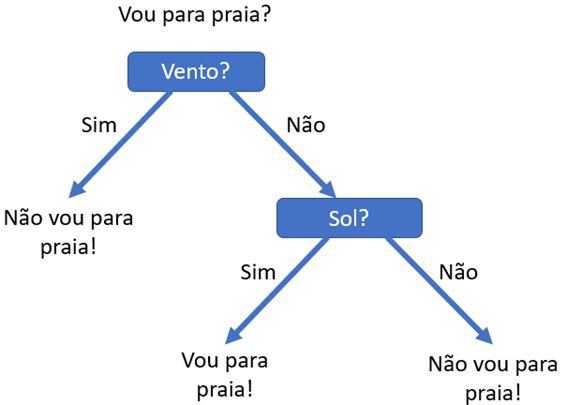
\includegraphics[width=7.3cm]{Images/image-5.png}
    \caption{Exemplo de uma estrutura de uma Árvore de Decisão}
    \label{fig:exampleFig1}
\end{figure}

\subsection{Floresta Aleatória}

Floresta Aleatória, (do inglês, \emph{Random Forest}) \cite{breiman2001random}, consiste basicamente da criação de diversas Árvores de Decisão de forma aleatória, ou seja, serão selecionados vários atributos de forma aleatória para iniciar a construção de cada árvore, de acordo com o parâmetro inicial dado (número de árvores de decisão a serem criadas). Após esta etapa, pode-se aplicar o treinamento do modelo, que fornecerá uma grande quantidade de métricas a serem analisadas, e que possivelmente serão apresentadas como uma média da acurácia obtida pelo conjunto de árvores, assim como é realizado neste trabalho.

\subsection{Gradient Boosting}

O \emph{Gradient Boosting} \cite{Friedman:99} é um método proveniente da área de Aprendizado de Máquina, cujo funcionamento tem grande suporte da técnica de \emph{boosting}, ou seja, podemos definí-lo de forma simplista como um classificador que utiliza uma combinação de resultados obtidos por preditores fracos (neste caso, Árvores de Decisão), para produzir resultados finais que possuem maior confiabilidade e desempenho em grande parte dos casos.

Apesar de ser identificado como um método \emph{Ensemble} como a Floresta Aletória, este utiliza a técnica de \emph{Boosting} em constraste com a técnica de \emph{Bagging} presente no \emph{Random Forest}. Isto significa que cada preditor fraco é classificado de forma sequencial e adaptativa, ou seja, existe dependência entre os modelos na etapa de treinamento. No treinamento de uma Floresta Aleatória, a execução deste processo acontece de forma pararela e independente, obtendo em grande parte dos casos como resultado final, uma média entre o conjunto de métricas.

\subsection{Validação Cruzada}

O método de validação cruzada (do inglês, \emph{k-fold}) \cite{CV}, consiste em dividir o conjunto total de dados em \(k\) subconjuntos mutuamente exclusivos de mesmo tamanho. A partir deste ponto, um subconjunto é utilizado para teste e os \(k - 1\) restantes são utilizados para treinamento, executando de forma cumulativa, os cálculos da acurácia do modelo. Este processo é realizado \(k\) vezes alternando de forma circular o subconjunto de teste, ou seja, aplicando o método \emph{holdout} de forma iterativa.

\subsection{Overfitting}

Overfitting (em português, \emph{sobre-ajustado}) \cite{Overfitting} caracteriza as situações em que o modelo "aprende demais" sobre os dados (se adequa de forma excessiva). Neste caso, o modelo mostra-se adequado apenas para os dados de treino, e não se mostra capaz de generalizar predições para um conjunto de dados nunca vistos antes. Quando isto acontece, os dados de treino apresentam resultados excelentes, enquanto a taxa de acerto do modelo descresce drasticamente com os dados de teste.

\section{Trabalhos Relacionados}

Embora tenha ocorrido uma intensa pesquisa sobre os recursos de Aprendizado de Máquina disponíveis para auxiliar no desenvolvimento deste trabalho, não encontramos até o momento, quaisquer outros trabalhos relacionados que pudessem nos fornecer bases de comparação entre métodos, e principalmente, resultados.

\section{Desenvolvimento do Trabalho}

Nas subseções à seguir, explanaremos de forma detalhada os processos que integraram o desenvolvimento deste trabalho, incluindo os obstáculos enfrentados na manipulação da base de dados, antes da etapa de aplicação do modelo de aprendizado em si.

\subsection{Base de Dados e Escolha dos Atributos} 

Este estudo utiliza a base de dados de Pokemóns \cite{Base} disponibilizada gratuitamente via Kaggle.

Este conjunto de dados contém informações sobre todos os 801 pokémons de todas as sete gerações de pokémon. As informações contidas neste conjunto de dados incluem dados básicos, desempenho contra outros tipos, altura, peso, classificação, etapas do ovo, valor de experiência, habilidade, etc.

\begin{figure}[H]
    \centering
    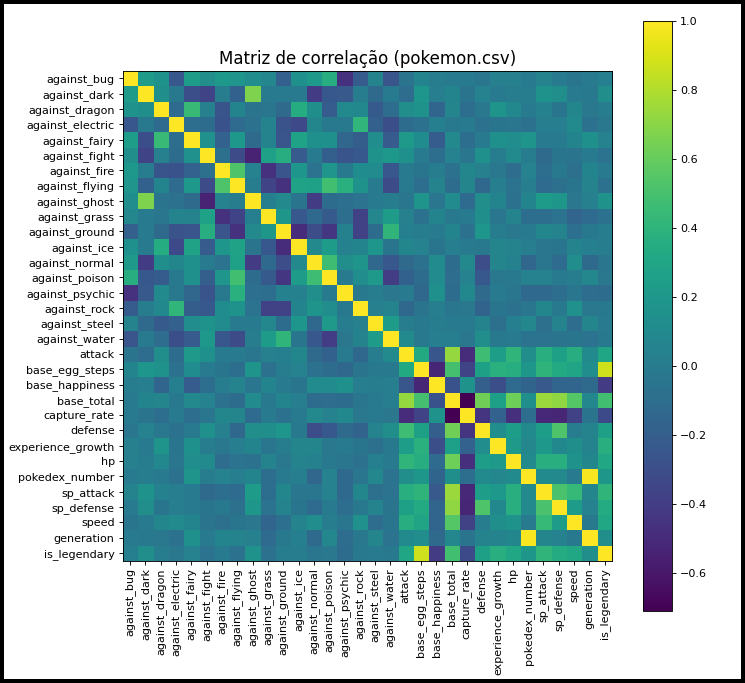
\includegraphics[width=14cm]{Images/correlation_matrix.png}
    \caption{Matriz de correlação da base de dados}
    \label{fig:exampleFig2}
\end{figure}

Ao todo a base possuí 40 atributos, sendo estes 39 preditores e 1 classe. A princípio, colocamos em uso todos os atributos disponíveis na base de dados, e realizamos os experimentos iniciais. É importante citar que utilizamos apenas o tipo primário do pokémon como classe, e por isso, o atributo \emph{type2} (tipo secundário) não foi introduzido no treinamento do modelo, embora este esteja presente na base de dados.

Na Figura~\ref{fig:exampleFig2} é apresentada a matriz de correlação referente aos atributos da base de dados e os graus de relação entre cada par. Atributos cujo quadrado de interseção tende ao amarelo, representam uma forte conexão, enquanto quadrados que tendem à cor azul, representam uma relação fraca ou inexistente entre o par de atributos.

\subsubsection{Perfil dos Atributos}

A seguir é apresentado um resumo dos atributos, informando seus nomes (rótulos) e o conteúdo típico que cada um armazena:

\begin{itemize}
    \item \emph{name}: Nome em inglês do pokémon;
    \item \emph{japanese\_name}: Nome em japonês do pokémon;
    \item \emph{pokedex\_number}: Número de entrada do pokémon na National Pokédex;
    \item \emph{percentage\_male}: Porcentagem das espécies que são machos. Não é atribuído valor caso o pokémon não possua gênero;
    \item \emph{classification}: A classificação do pokémon conforme descrito pelo Sun e Moon Pokédex;
    \item \emph{height\_m}: Altura do pokémon em metros;
    \item \emph{weight\_kg}: O peso do pokémon em quilogramas;
    \item \emph{capture\_rate}: Taxa de captura do pokémon;
    \item \emph{baseeggsteps}: O número de passos necessários para chocar um ovo do pokémon;
    \item \emph{abilities}: Uma lista de habilidades que o pokémon pode possuir;
    \item \emph{experience\_growth}: A taxa de crescimento da experiência do pokémon;
    \item \emph{base\_happiness}: Felicidade base do pokémon;
    \item \emph{against\_\(<\)type\(>\)}: Dezoito recursos que denotam a quantidade de dano recebido contra ataques de determinado tipo de pokémon;
    \item \emph{hp}: A vida base do pokémon;
    \item \emph{attack}: O dano de ataque base do pokémon;
    \item \emph{defense}: Defesa base do Pokémon;
    \item \emph{sp\_attack}: O ataque especial base do pokémon;
    \item \emph{sp\_defense}: A base especial de Defesa do pokémon;
    \item \emph{speed}: A velocidade base do pokémon;
    \item \emph{generation}: A geração numerada em que o Pokémon foi introduzido pela primeira vez;
    \item \emph{is\_legendary}: Indica se o Pokémon é lendário.
\end{itemize}

\subsubsection{Perfil da Classe}

A classe que desejamos trabalhar nas predições do modelo é apresentada abaixo:

\begin{itemize}
    \item \emph{type1}: O tipo primário do Pokémon.
\end{itemize}

\subsection{Metodologia}

Neste trabalho, optamos pela utilização da biblioteca Python \emph{scikit-learn} para implementar o modelo de aprendizado. Dentre os vários métodos de aprendizado de máquina existentes, selecionamos a Árvore de Decisão (do inglês, \emph{Decision Tree}), Floresta Aleatória (do inglês, \emph{Random Forest}) e  Gradient Boosting para formular o modelo de predições. A implementação encontra-se disponível publicamente em \url{https://github.com/juliorodrigues07/TP-1-Machine-Learning}.

Esta escolha se deve à versatilidade destes métodos, que podem ser aplicados em problemas de classificação e regressão, obtendo resultados satisfatórios em grande parte dos casos. Vale citar também a facilidade de aplicação dos mesmos, utilizando as implementações prontas da biblioteca, além da complexidade inferior para lidar com classes que possuem múltiplos rótulos como a utilizada neste trabalho.

Além disso, foram utilizadas bibliotecas auxiliares como \emph{Matplotlib} \cite{Matplotlib} e \emph{pandas} \cite{pandas}, para construção de gráficos relacionados ao aprendizado do modelo e leitura da base de dados, respectivamente.

\subsection{Pré-Processamento}

Ao longo do desenvolvimento do trabalho, nos deparamos com algumas adversidades antes de avançar para a fase de execução do modelo de aprendizado em si. Estes obstáculos, em sua grande parte, estavam relacionados ao tratamento da base de dados, esta que apresentava algumas inconsistências que impossibilitavam a aplicação dos recursos que a biblioteca \emph{scikit-learn} oferece. Portanto, fez-se necessário a aplicação de algumas ferramentas de pré-processamento, para que se fizesse possível a implementação de um modelo de aprendizado de máquina.

O primeiro obstáculo encontrado na implementação do modelo, foi a limitação existente no algoritmo que implementa a Árvore de Decisão na biblioteca. Na \emph{scikit-learn}, o método é implementado utilizando uma versão otimizada do algoritmo \emph{CART} \cite{CART}, que por sua vez, é um derivado do algoritmo \emph{C4.5}. A principal "falha" \hspace{0.01cm} no modo de operação deste algoritmo, é que este não é capaz de lidar com valores categóricos (nominais) para realizar as etapas de treinamento e predições.

A solução encontrada para esta limitação, foi a aplicação de um processo de discretização dos valores categóricos que alguns atributos da base e a classe apresentam (abilities, classification, japanese\_name, name e type1). Basicamente, o que ocorre nesta execução é atribuição de um valor inteiro para cada valor categórico distinto na base. Então, utilizando a classe como exemplo, aos dezoito tipos de pokémon (fire, water, psyquic...) vão ser atribuídos os valores de 0 a 17, de acordo com a ordem em que estes ocorrem na base de dados.

Outro obstáculo encontrado na utilização correta da base de dados, deve-se a mesma apresentar a ausência de valores para alguns atributos, o que exigiu a aplicação de uma estratégia para preenchimento de valores ausentes (do inglês, \emph{missing values}). Entre os recursos disponíveis, optamos por atributir a média da distribuição de cada atributo na base para o conjunto de valores ausentes. Vale citar também que utilizamos um recurso de escalonamento disponível na biblioteca, que não vamos detalhar neste artigo, mas que teve sua utilidade para ajustar a distribuição da base de dados.

Por fim, devido a complexidade e quantidade de informações que a base apresenta (39 atributos e 1 classe com 18 rótulos), decidimos por aplicar um processo de seleção dos atributos que possuem as maiores relevâncias na formulação do modelo de aprendizado, utilizando os recursos oferecidos pela biblioteca \emph{scikit-learn}. 

Basicamente, o que realizamos foi o treinamento de várias árvores de decisão "extras" para encontrar atributos cujo ganho de informação era nulo ou muito pequeno, utilizando entropia como critério. Dados tais atributos menos relevantes, executamos seu descarte para obter uma base de dados mais compacta, o que implicou em um desempenho melhor por parte dos modelos de aprendizado treinados, além de diminuir suas complexidades, ambos aspectos que serão discutidos mais adiante neste artigo.

\subsection{Aplicação dos Métodos}

Após a aplicação da etapa de pré-processamento explanada na seção 4.4, pode-se dizer que a base estava integralizada para ser trabalhada na aplicação dos métodos de aprendizado de máquina.

Ao todo, a base foi manipulada de quatro formas distintos para aferir o aprendizado. Estas são, a modelagem utilizando uma árvore de decisão ordinária, uma floresta aleatória, e por fim, testes \emph{holdout} e também utilizando validação cruzada (do inglês, \emph{cross-validation}) com as mesmas.

Na utilização da Árvore de Decisão ordinária, aplicando \emph{entropia} como critério para realizar a modelagem, utilizamos instâncias previamente selecionadas para treinamento, estas que correspondem à 80\% da base de dados total (20\% restantes utilizados para teste).

Para a aplicação da Floresta Aleatória, também definindo a \emph{entropia} como critério, construímos um conjunto com cem Árvores de Decisão, cujo desempenho apresentou resultados ligeiramente melhores que a utilização de uma única árvore de decisão. A aplicação destes métodos, resultados e análise, serão explorados na seção 5 a seguir.

Quanto ao Gradient Boosting, após a finalização de uma bateria de testes para treinamento do modelo, definimos como hiperparâmetros a taxa de aprendizado fixada em 0,3 e a profundidade máxima em 5, o que apresentou resultados superiores ao treinamento de uma árvore de decisão única, mas ligeiramente inferiores aos obtidos pela floresta aleatória. 

Pom fim, para a aplicação da validação cruzada, definimos como \(k\) o valor 10, ou seja, a base é dividida dez vezes em porções que serão escalonadas entre treinamento e teste coletando as pontuações de acurácia. Ao final deste processo, o resultado será a média destas pontuações. Vale ressaltar que a utilização desta técnica tem grande utilidade na análise de \emph{underfitting} e \emph{overfitting} que podem ocorrer no modelagem do software preditor. A partir deste ponto, vamos nos referir a validação cruzada como \emph{CV} no restante deste artigo.

\section{Experimentos Iniciais e Análise dos Resultados}

Uilizando a implementação da Árvore de Decisão disponível na biblioteca \emph{scikit-learn}, ausente de quaisquer refinamentos de parâmetros (podas, fator de ramificação e profundidade máxima, por exemplo), conseguimos gerar a árvore ilustrada na Figura~\ref{fig:exampleFig3}.

Podemos observar uma árvore bastante complexa, cujo número de nós e a profundidade são bastante elevados devido às dezenas de atributos com os quais o modelo teve que lidar, além da classe multirótulo, com dezoito tipos distintos de pokémon presentes.

\begin{figure}[H]
    \centering
    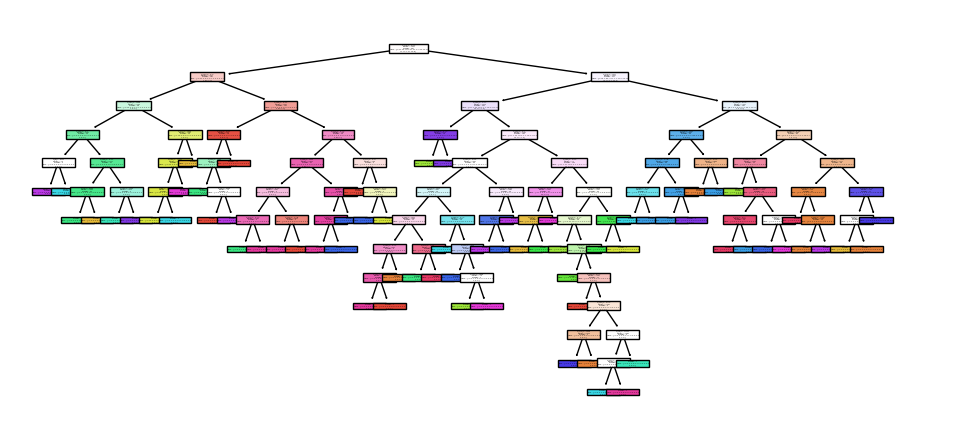
\includegraphics[width=16cm]{Images/arvore_de_decisao.png}
    \caption{Árvore de Decisão gerada pelo algoritmo}
    \label{fig:exampleFig3}
\end{figure}

\vspace{4.2cm}
\subsection{Árvore de Decisão com e sem CV}

Utilizando testes ordinários, onde se divide a base em um subconjunto de treinamento e outro para testes, obtivemos como aproveitamento 86,96\% de acurácia em média. É importante ressaltar que nestes testes ordinários, dividimos a base em 80\% dos dados para treinamento, os 20\% restante para testes. Utilizando proporções razoáveis como esta, podemos diminuir o risco de ocorrência de \emph{underfitting} ou \emph{overfitting} em grande parte dos problemas.

Na abordagem utilizando CV, como citado anteriormente, a base é dividida dez vezes em subconjuntos que serão escalonados entre treinamento e teste, resultando em uma lista de valores que correspondem à acurácia atingida pelo classificador em cada divisão. Portanto, utilizando esta técnica, obtivemos como resultado uma média de 83,14\% de acurácia nas predições. 

À seguir, serão apresentadas na Tabela~\ref{tab:exampleTab1} e na Figura~\ref{fig:exampleFig5}, um resumo das métricas obtidas na etapa de predições, executando testes ordinários e gerando a matriz de confusão obtida na aplicação dos mesmos, apresentando valores absolutos e possibilitando comparações entre as predições realizadas pelo classificador e os tipos verdadeiros (Falsos positivos e negativos). O gráfico das curvas de aprendizado também é exibido à seguir na Figura~\ref{fig:exampleFig4}:

\begin{figure}[H]
    \centering
    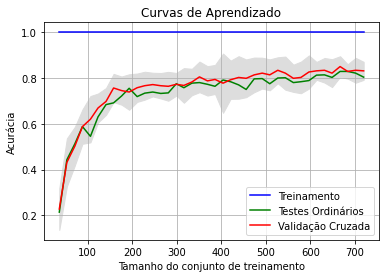
\includegraphics[width=0.8\textwidth]{Images/learning_curves_tree.png}
    \caption{Curvas de Aprendizado da Árvore de Decisão}
    \label{fig:exampleFig4}
\end{figure}

\begin{table}[H]
    \centering
    \caption{Métricas obtidas nos testes para predições cada rótulo}
    \label{tab:exampleTab1}
    \begin{tabular}{c|c|c|c|c}
                    &   Precision &  Recall   & f1score   & support\\ 
        bug         &      0,80   &   0,84    &  0,82     &   19\\
        dark        &      1,00   &   0,33    &  0,50     &    3\\
        dragon      &      1,00   &   0,33    &  0,50     &    3\\
        electric    &      1,00   &   1,00    &  1,00     &    9\\
        fairy       &      1,00   &   1,00    &  1,00     &    4\\
        fighting    &      0,71   &   0,83    &  0,77     &    6\\
        fire        &      1,00   &   0,77    &  0,87     &   13\\
        flying      &      0,00   &   0,00    &  0,00     &    0\\
        ghost       &      0,83   &   0,83    &  0,83     &    6\\
        grass       &      0,94   &   1,00    &  0,97     &   17\\
        ground      &      0,86   &   1,00    &  0,92     &    6\\
        ice         &      1,00   &   0,80    &  0,89     &    5\\
        normal      &      0,91   &   0,95    &  0,93     &   22\\
        poison      &      1,00   &   0,57    &  0,73     &    7\\
        psyquic     &      0,62   &   0,71    &  0,67     &    7\\
        rock        &      0,70   &   1,00    &  0,82     &    7\\
        steel       &      0,67   &   0,50    &  0,57     &    4\\\vspace{0.5cm}
        water       &      0,92   &   1,00    &  0,96     &   23\\
        accuracy    &        -    &     -     &  0,87     &  161\\
        macro avg   &      0,83   &   0,75    &  0,76     &  161\\
        weighted avg &     0,89   &   0,87    &  0,87     &  161
    \end{tabular}
\end{table}

\begin{figure}[H]
    \centering
    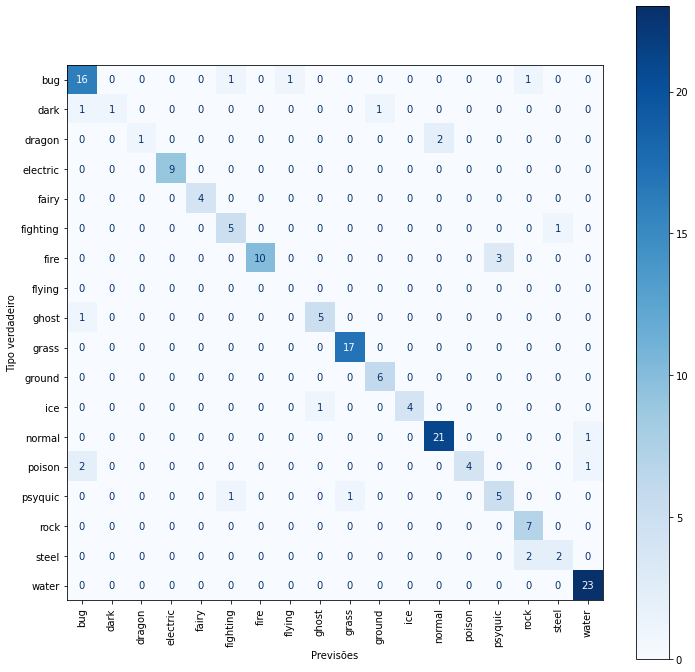
\includegraphics[width=0.95\textwidth]{Images/confusion_matrix_tree.png}
    \caption{Matriz de Confusão para testes com Árvore de Decisão}
    \label{fig:exampleFig5}
\end{figure}

Podemos observar que grande parte do conjunto de teste foi classificado na forma correta pelo modelo de aprendizado, ou seja, a diagonal principal apresenta a maior concentração dos dados, característica que nos fornece um indício de que o modelo construído não está apresentando \emph{overfitting}.

\subsection{Floresta Aleatória com e sem CV}

Para testes ordinários, em que geramos cem árvores de decisão, obtivemos como aproveitamento 92,55\% de acurácia em média. Em testes com validação cruzada, assim como na utilização da Árvore de Decisão "pura", este valor sofreu um leve declínio, apresentando como resultado uma acurácia média de 88,63\%. Vale citar que a implementação da Floresta Aleatória excluiu instâncias do tipo \emph{flying} (No total só existem duas na base). Não sabemos exatamente o porque desta exclusão, mas parece que o método pode ter identicado tais instâncias como \emph{outliers} extremos, e então as removeu do modelo.

O resumo das métricas obtidas na etapa de predições, executando testes ordinários é exibido na Tabela~\ref{tab:exampleTab2} à seguir:

\begin{table}[H]
    \centering
    \caption{Métricas obtidas nos testes para predições cada rótulo}
    \label{tab:exampleTab2}
    \begin{tabular}{c|c|c|c|c}
                    &   Precision &  Recall   & f1score   & support\\ 
        bug         &      0,94   &   0,84    &  0,89     &   19\\
        dark        &      1,00   &   0,67    &  0,80     &    3\\
        dragon      &      1,00   &   1,00    &  1,00     &    3\\
        electric    &      1,00   &   1,00    &  1,00     &    9\\
        fairy       &      1,00   &   1,00    &  1,00     &    4\\
        fighting    &      0,71   &   0,83    &  0,77     &    6\\
        fire        &      0,87   &   1,00    &  0,93     &   13\\
        ghost       &      0,71   &   0,83    &  0,77     &    6\\
        grass       &      0,94   &   1,00    &  0,97     &   17\\
        ground      &      0,86   &   1,00    &  0,92     &    6\\
        ice         &      1,00   &   0,80    &  0,89     &    5\\
        normal      &      1,00   &   0,91    &  0,95     &   22\\
        poison      &      1,00   &   1,00    &  1,00     &    7\\
        psyquic     &      1,00   &   0,71    &  0,83     &    7\\
        rock        &      1,00   &   1,00    &  1,00     &    7\\
        steel       &      0,67   &   1,00    &  0,80     &    4\\\vspace{0.5cm}
        water       &      0,96   &   0,96    &  0,96     &   23\\
        accuracy    &        -    &     -     &  0,93     &  161\\
        macro avg   &      0,92   &   0,92    &  0,91     &  161\\
        weighted avg &     0,94   &   0,93    &  0,93     &  161
    \end{tabular}
\end{table}

O gráfico das curvas de aprendizado (Figura~\ref{fig:exampleFig6}) é exibido à seguir:

\begin{figure}[H]
    \centering
    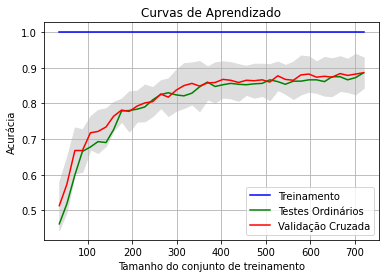
\includegraphics[width=0.8\textwidth]{Images/learning_curves_forest.png}
    \caption{Curvas de Aprendizado da Floresta Aleatória}
    \label{fig:exampleFig6}
\end{figure}

A matriz de confusão (Figura~\ref{fig:exampleFig7}), apresentando valores absolutos e possibilitando comparações entre as predições realizadas pelo classificador e os tipos verdadeiros, é exibida à seguir:

\begin{figure}[H]
    \centering
    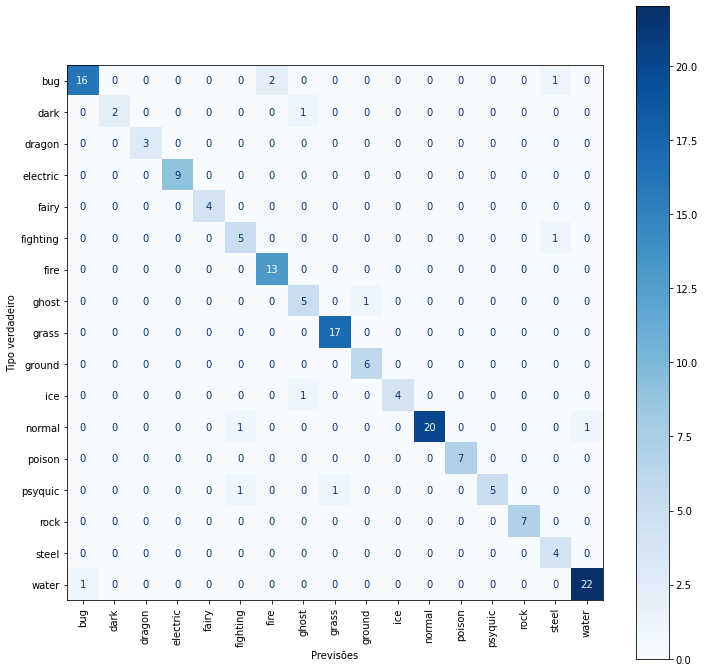
\includegraphics[width=0.9\textwidth]{Images/confusion_matrix_forest.png}
    \caption{Matriz de Confusão para testes com Floresta Aleatória}
    \label{fig:exampleFig7}
\end{figure}

\vspace{1.5cm}
\subsection{Gradient Boosting com e sem CV}

Para testes ordinários, em que geramos cem árvores de decisão, obtivemos como resultado 91,92\% de acurácia em média. Em testes com validação cruzada, assim como na aplicação dos outros dois métodos citados anteriormente, esta métrica sofreu um leve declínio, apresentando como resultado uma acurácia média de 87,76\%. Assim como na aplicação da Floresta Aleatória, o método excluiu automaticamente exemplos do tipo \emph{flying}.

Os detalhes das métricas obtidas na etapa de predições executando testes ordinários é exibido na Tabela~\ref{tab:exampleTab3} à seguir:

\begin{table}[H]
    \centering
    \caption{Métricas obtidas nos testes para predições cada rótulo}
    \label{tab:exampleTab3}
    \begin{tabular}{c|c|c|c|c}
                    &   Precision &  Recall   & f1score   & support\\ 
        bug         &      0,89   &   0,89    &  0,89     &   19\\
        dark        &      0,67   &   0,67    &  0,67     &    3\\
        dragon      &      1,00   &   1,00    &  1,00     &    3\\
        electric    &      0,90   &   1,00    &  0,95     &    9\\
        fairy       &      1,00   &   1,00    &  1,00     &    4\\
        fighting    &      1,00   &   0,83    &  0,91     &    6\\
        fire        &      0,86   &   0,92    &  0,89     &   13\\
        ghost       &      0,75   &   1,00    &  0,86     &    6\\
        grass       &      0,94   &   1,00    &  0,97     &   17\\
        ground      &      1,00   &   1,00    &  1,00     &    6\\
        ice         &      1,00   &   0,80    &  0,89     &    5\\
        normal      &      1,00   &   0,95    &  0,98     &   22\\
        poison      &      0,83   &   0,71    &  0,77     &    7\\
        psyquic     &      1,00   &   0,86    &  0,92     &    7\\
        rock        &      0,88   &   1,00    &  0,93     &    7\\
        steel       &      0,67   &   0,50    &  0,57     &    4\\\vspace{0.5cm}
        water       &      0,96   &   0,96    &  0,96     &   23\\
        accuracy    &        -    &     -     &  0,92     &  161\\
        macro avg   &      0,90   &   0,89    &  0,89     &  161\\
        weighted avg &     0,92   &   0,92    &  0,92     &  161
    \end{tabular}
\end{table}

O gráfico das curvas de aprendizado (Figura~\ref{fig:exampleFig8}) é exibido à seguir:

\begin{figure}[H]
    \centering
    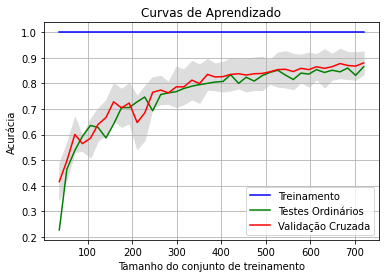
\includegraphics[width=0.8\textwidth]{Images/learning_curves_gradient.png}
    \caption{Curvas de Aprendizado da Gradient Boosting}
    \label{fig:exampleFig8}
\end{figure}

A matriz de confusão (Figura~\ref{fig:exampleFig9}), apresentando valores absolutos e possibilitando comparações entre as predições realizadas pelo classificador e os tipos verdadeiros, é exibida à seguir:

\begin{figure}[H]
    \centering
    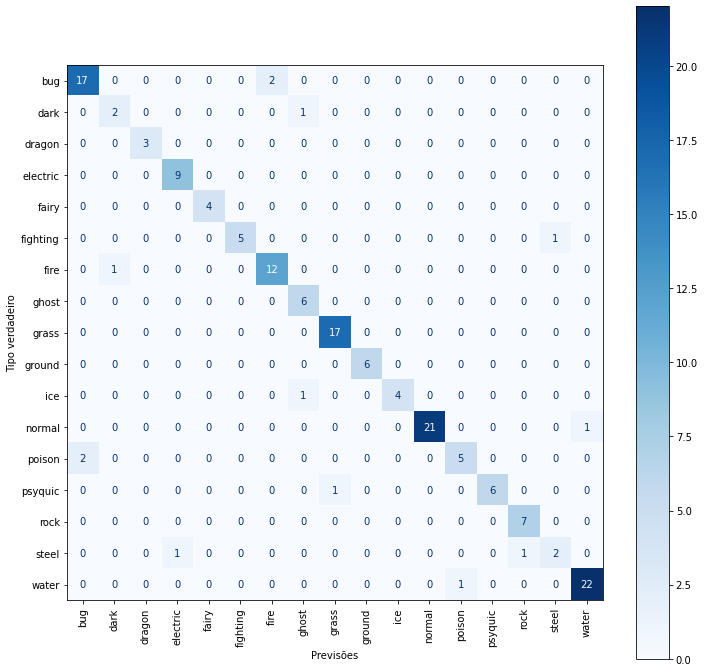
\includegraphics[width=0.9\textwidth]{Images/confusion_matrix_gradient.png}
    \caption{Matriz de Confusão para testes com Gradient Boosting}
    \label{fig:exampleFig9}
\end{figure}

\subsection{Resultados}

Se encontram na Tabela~\ref{tab:exampleTab4} e Tabela~\ref{tab:exampleTab5} de forma resumida e clara, as acurácias obtidas na aplicação de cada método, de acordo com os modos de teste empregados na implementação do modelo de aprendizado, antes e depois da aplicação da técnica de descarte de atributos menos relevantes, mecionada na seção sobre pré-processamento da base de dados.

\begin{table}[H]
    \centering
    \caption{Acurácias obtidas antes da remoção de atributos menos relevantes}
    \label{tab:exampleTab4}
    \begin{tabular}{c|c|c}
        Algoritmo & Teste Ordinário & Validação Cruzada \\ 
        Árvore de Decisão & 85,7\% & 83\%\\
        Floresta Aleatória & 88,82\% & 86,4\%\\
        Gradient Boosting & 89,44\% & 88\%
    \end{tabular}
\end{table}

\begin{table}[H]
    \centering
    \caption{Acurácias obtidas depois da remoção de atributos menos relevantes}
    \label{tab:exampleTab5}
    \begin{tabular}{c|c|c}
        Algoritmo & Teste Ordinário & Validação Cruzada \\ 
        Árvore de Decisão & 86,96\% & 83,14\%\\
        Floresta Aleatória & 92,55\% & 88,63\%\\
        Gradient Boosting & 91,92\% & 87,76\%
    \end{tabular}
\end{table}

\section{Considerações Finais}

Por fim, concluímos dessa forma a segunda fase de desenvolvimento deste trabalho, que possibilitou a expansão de nosso conhecimento no ramo de aplicações de métodos de aprendizado de máquina, assim como seus graus de importância na resolução de problemas mais complexos e delicados do mundo real, os quais demandam e permitem ainda mais o avanço da tecnologia.

Observando os testes apresentados, podemos concluir que a acurácia da Árvore de Decisão (preditor fraco), em um contexto onde há muito atributos, é inferior aos resultados obtidos pelos métodos \emph{Ensemble} (Floresta Aleatória e Gradient Boosting). Contudo, é importante ressaltar que apesar de obter uma acurácia superior, a Floresta Aleatória, e principalmente o Gradient Boosting, possuem um custo computacional bem superior ao apresentado pela Árvore de Decisão. 

Embora os resultados obtidos possam ser considerados como adequados, dado o número de exemplos presentes na base de dados, ainda existem certas lacunas para melhoria, como no aprimoramento da etapa de pré-processamento. Sabemos que a base de dados apresenta um conjunto de exemplos cuja classe é bastante desbalanceada. Para contornar este obstáculo, poderíamos tentar expandir o conjunto de exemplos com instâncias virtuais (fictícias, adequando-se aos atributos daquele rótulo), ou até mesmo realizar a união classes que ocupam as menores proporções na base, possibilitando novas etapas de treinamento do modelo, e possivelmente a obtenção de melhores resultados.

\bibliographystyle{sbc}
\bibliography{A.bib}

\end{document}

